
\chapter{Description de l'API de \PpFf}
\label{description.chap}

\gt{Pour \'eviter la confusion, tu dois utiliser les m\^emes termes
que dans l'API, m\^eme si ces termes sont en anglais. Mais tu les mets
dans la police courrier, avec texttt.}

\GT{Pas besoin de mettre API en \TT{API} --- c'est un acronyme, pas un
identificateur provenant du code source. Idem pour STL.}

\begin{figure}[ht]
\centering
     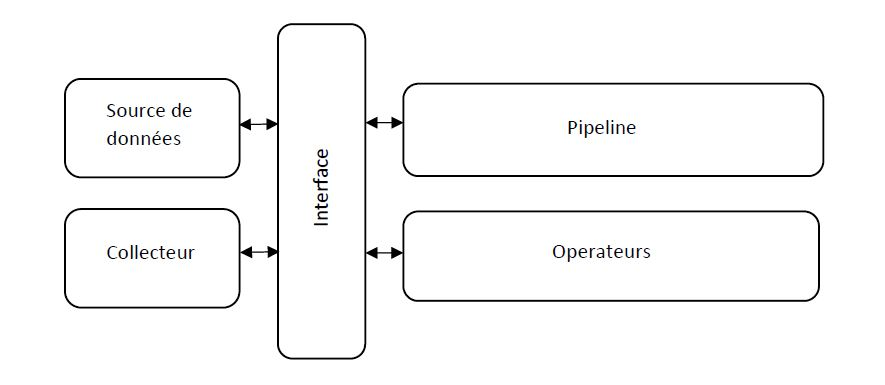
\includegraphics[width=1.0\textwidth]{Figures/ComponentsAPI.jpg}
      \caption{Les composants de l'API de \ppff.}
       \label{ComponentsAPI.fig}
\end{figure}


\GT{Pour ce premier diagramme de classes: il ne faudrait mettre que
les classes qui sont visibles aux utilisateurs, donc les <<concepts>>
qui sont utiles pour utiliser l'API et \^etre capable de s'en
servir. Les autres classes de plus bas niveau (en lien avec FastFlow
par exemple), pourront \^etre pr\'esent\'ees dans le prochain
chapitre.}


Ce chapitre pr\'esente l'API de \ppff. Sa conception permet aux utilisateurs de tirer parti de la simplicit\'e d'utilisation tout en cachant la complexit\'e concernant les m\'ecanismes concurrents utilis\'es. La figure~\ref{ComponentsAPI.fig} pr\'esente une vue d'ensemble de l'architecture de \ppff. L'API est compos\'ee de quatre \'el\'ements principaux: l'Interface avec laquelle le d\'eveloppeur interagit, les \TT{Pipeline}s --- qui sont le coeur de l'API ---, les \TT{Stage}s et les \TT{Operator}s. Le r\^ole de chaque composant dans l'API est pr\'esent\'e dans la section suivante. La derni\`ere section  d\'ecrit plus en d\'etail les principales m\'ethodes de l'interface.

% \GT{La macro \PpFf{} permet de g\'en\'erer la forme correcte, et
% partout pareille. Une version sans majuscule, plus simple \`a
% utiliser, produit la m\^eme chose.}

L'{API} de \PpFf{} est impl\'ement\'e au-dessus de la biblioth\`eque \TT{FastFlow}, impl\'ementation qui sera d\'ecrite au prochain chapitre.

Le pr\'esent chapitre d\'ecrit le r\^ole de chaque composant de
\PpFf{}. La figure~\ref{ClassDiagramme.jpg} pr\'esente une vue
d'ensemble des classes qui composent l'{API}.

\GT{<<et leur mappage aux mod\`eles de \TT{FastFlow}>>: Non, dans
le prochain chapitre, pas dans celui-ci!}

%
%\GT{Probablement qu'un diagramme de classe UML serait int\'eressant et
%utile.  Il pourrait \^etre introduit ici, puis expliqu\'e dans les
%sous-sections qui suivent.}
%
%\GT{Note que de fa\c{c}on g\'en\'erale, lorsqu'on d\'ebute une section
%qui contient plusieurs sous-sections, il est pr\'ef\'erable d'avoir
%quelques lignes d'introduction, qui donnent une vue d'ensemble de ce
%qui suit. Pas toujours, mais ici, avec le diagramme de classes, \c{c}a
%ferait l'affaire.}
%
%\IC{Mon plan initial \'etait de d\'ecrire les composants dans le chapitre 2 (Description de l'API de \PpFf) et de pr\'esenter la partie technique dans le chapitre 3 (Impl\'ementation). Dans la premi\`ere partie du chapitre 2 j'ai choisi de d\'ecrire les composants principaux de l'API et dans la deuxi\`eme partie de ce chapitre de pr\'esenter quelques m\'ethodes avec des exemples. 
%Dans le chapitre 3 j'ai eu l'intention d'introduire un diagramme de classe UML en expliquant les classes qui compose l'API. } 
%
%\IC{Qu'est-ce que vous en pensez ? Est-ce que je dois introduire le diagramme dans le chapitre 2 ? Je ne suis pas sûr que je fasse la différence entre la description et implémentation de l’API.
%}


%\GT{La description est tout ce qu'un programmeur doit savoir/connaitre
%pour \underline{utiliser} ton API --- de l'ext\'erieur, comme une
%boite noire. L'impl\'ementation d\'ecrit les <<d\'etails>>
%n\'ecessaires pour comprendre \underline{comment fonctionne} l'API,
%par exemple, ce qu'un mainteneur devrait comprendre/connaitre s'il
%voulait modifier, corriger ou \'etendre ton API.}
%
%\GT{En lien avec le diagramme de classes, si l'utilisateur de l'API
%utilise ou manipule diff\'erents concepts et classes dans son
%programme, que ces concepts/classes sont utiles pour pouvoir utiliser
%correctement l'API --- avec la bonne syntaxe et la bonne s\'emantique
%--- alors ces concepts devraient \^etre d\'ecrits, par un diagramme de
%classes par exemple.}

\section{Interface}

\begin{figure}[ht]
\centering
     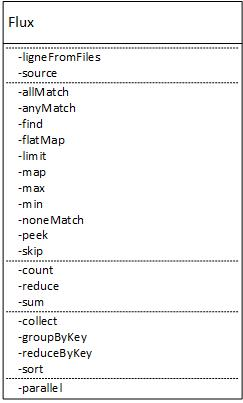
\includegraphics[width=1.0\textwidth]{Figures/ClassDiagramme.jpg}
      \caption{Les classes qui composent l'{API}.}
       \label{ClassDiagramme.fig}
\end{figure}


L'interface propos\'ee en \PpFf\ consiste en un ensemble de m\'ethodes qui permettent \`a l'utilisateur de manipuler des flux de donn\'ees de mani\`ere simple et efficace. L'interface suit d'assez pr\`es celle introduite pour les \emph{Streams} de Java~8. Le tableau~\ref{methodes_api.tab} d\'ecrit bri\`evement les m\'ethodes impl\'ement\'ees dans l'API.




%\GT{Dans un tabular, pour mettre du texte, on utilise p avec une
%largeur. Ceci \'evite de mettre des sauts de lignes explicites, ce qui
%n'est jamais une bonne id\'ee.}

%\GT{Il faut mettre le code avec police tt. Par contre, j'ai essay\'e
%que le code soit mis par d\'efaut ainsi, mais cela n'a pas
%fonctionn\'e, d'o\`u les commandes tt ins\'er\'ees en d\'ebut de
%chaque ligne~:(}
%
%\GT{Par contre, le d\'efaut avec la solution actuelle, c'est que c'est
%tr\`es difficile \`a comprendre pour les m\'ethodes plus complexes. Il
%faudra qu'on r\'efl\'echisse \`a une fa\c{c}on plus claire de
%pr\'esenter la signaure des m\'ethodes.}
%
%\IC{J'ai ajout\'e toutes les m\'ethodes d\'efinies dans l'interface de l'API dans ce tableau et j'ai \'et\'e oblig\'e d'utiliser le paquet longtable parce qu'elle s'\'etendait sur plusieurs pages. J'ai essay\'e de pr\'esenter la signature des m\'ethodes dans un format plus concis. Par exemple le paramètre std ::fonction a \'et\'e remplac\'e pour Func; j'ai enlev\'e les mots typename de chaque d\'eclaration de template; le param\`etre <typename ELEM, class ALLOC = std ::allocator<ELEM class TContainer >> a \'et\'e remplac\'e pour Container. De plus je n'ai pas pu r\'eutiliser la fonction qui redimensionne le tableau resizebox(textwidth). J'ai utilis\'e une police de caract\`ere plus petite (tiny) pour pouvoir encadrer le tableau dans la page.
%}
%
%\IC{J'ai reformul\'e la description pour le r\'esultat de la fonction flatMap}


%\begin{landscape}
\newpage
\KOMAoptions{paper=landscape,pagesize}
\recalctypearea


\begin{center}
\footnotesize
\begin{longtable}{|l|l|p{5cm}|}
\caption{Les m\'ethodes publiques de l'API de~\ppff.\label{methodes_api.tab}}\\
\hline
\textbf{M\'ethode} & \textbf{Type du r\'esultat} & \textbf{Description du r\'esultat}\\
\hline
\endfirsthead
\multicolumn{3}{c}%
{\tablename\ \thetable\ Méthodes publiques de l'API (\textit{suite})} \\
\hline
\textbf{M\'ethode} & \textbf{Type du r\'esultat} & \textbf{Description du r\'esultat}\\
\hline
\endhead
\hline \multicolumn{3}{r}{\textit{Suite page suivante}} \\
\endfoot
\hline
\endlastfoot
\hline
	\begin{tabular}{@{}l@{}}
	\tt template<T> \\
	\tt allMatch(Func<bool(T*)> predicate)
	\end{tabular} &
  	\TT{bool} &
    Retourne \TT{true} si tous les \'el\'ements
    du flux satisfont \TT{predicate}, sinon \TT{false}.
    \\
\hline
	\begin{tabular}{@{}l@{}}
	\tt template<T> \\
	\tt anyMatch(Func<bool(T*)> predicate)
	\end{tabular} &
  	\TT{bool} & 
    Retourne \TT{true} si au moins un  
    \'el\'ement du flux satisfait \TT{predicate}, sinon \TT{false}.
\\
\hline
	\begin{tabular}{@{}l@{}}
	\tt template<T, Container<T>{>}\\
	\tt collect()
	\end{tabular} &
  	\TT{Container<T>} &
    Retourne un conteneur
    STL avec tous les \'el\'ements du flux.
    \\
\hline
	\begin{tabular}{@{}l@{}}
	\tt count()\\
	\end{tabular} &
  	\TT{unsigned int} & 
    Retourne le nombre d'\'el\'ements
    du flux.
    \\
\hline
	\begin{tabular}{@{}l@{}}
	\tt template<In> \\
	\tt find(Func<bool(In*)> const\& predicate)
	\end{tabular} &
  	\TT{Pipe\&} &
    Retourne les
    \'el\'ements du flux qui satisfont \TT{predicate}.
    \\
\hline
	\begin{tabular}{@{}l@{}}
	\tt template<In, Out, Container> \\
	\tt flatMap(Func<Container*(In*)> const\& taskFunc)
	\end{tabular} &
  	\TT{Pipe\&} & 
    Applique la fonction fournie en argument
    \`a chaque \'el\'ement du flux et concat\`ene ces \'el\'ements lorsque plusieurs sont produits par la fonction.
    \\
\hline
	\begin{tabular}{@{}l@{}}
	\tt template<In, Out, Container=In> \\
	\tt flatMap()
	\end{tabular} &
  	\TT{Pipe\&} &
    Produit un flux avec les \'el\'ements du conteneur.  
    \\
\hline
	\begin{tabular}{@{}l@{}}
	\tt template<In, K=In, V=In, MapType> \\
	\tt groupByKey(Func<K*(In*)> fk, Func<V*(In*)> fv)
	\end{tabular} &
  	\TT{MapType} &
    Retourne un dictionnaire (\emph{map}) avec les \'el\'ements
    du flux regroupés par cl\'e.
   \\
\hline
%	\begin{tabular}{@{}l@{}}
%	\tt template<T, Container> \\
%	\tt intermediateCollect()
%	\end{tabular} &
%	\TT{Collection<T, Container>} &
%    Retourne une collection avec les
%    \'el\'ements du flux. \GT{Est-ce utile de mentionner cette m\'ethode?}
%    \\ 
%\hline
	\begin{tabular}{@{}l@{}}
	\tt template<T> \\
	\tt limit(int n)
	\end{tabular} &
	\TT{Pipe\&} & 
    Retourne un flux compos\'e des \TT{n}~premiers \'el\'ements du flux d'entr\'ee.
    \\
\hline
	\begin{tabular}{@{}l@{}}
	\tt linesFromFile(string\& path)
	\end{tabular} &
	\TT{Pipe\&} & 
    Retourne un flux avec les lignes
    contenues dans le fichier indiqu\'e par \TT{path}.
    \\
\hline
	\begin{tabular}{@{}l@{}}
	\tt template<In, Out> \\
	\tt map(Func<Out*(In*)> const\& taskFunc)
	\end{tabular} &
	\TT{Pipe\&} & 
    Retourne un flux compos\'e de
    l'application de \TT{taskFunc}
    \`a chacun des
    \'el\'ements du flux.
    \\
\hline
	\begin{tabular}{@{}l@{}}
	\tt template<T> \\
	\tt max(Func<void(T*, T*)> compare)
	\end{tabular} &
	\TT{T} &
	Retourne l'\'el\'ement maximum du flux en fonction du comparateur.
    \\
\hline
	\begin{tabular}{@{}l@{}}
	\tt template<T> \\
	\tt min(Func<void(T*, T*)> compare)
	\end{tabular} &
	\TT{T} &
	Retourne l'\'el\'ement minimum du flux en fonction du comparateur.
    \\
\hline
	\begin{tabular}{@{}l@{}}
	\tt template<T> \\
	\tt noneMatch(Func<bool(T*)> predicate)
	\end{tabular} &
	\TT{bool} &
    Retourne \TT{true} si aucun des \'el\'ements
    du flux ne satisfait \TT{predicate},
    sinon \TT{false}.
    \\
\hline
	\begin{tabular}{@{}l@{}}
	\tt parallel(int workers = 1)
	\end{tabular} &
	\TT{Pipe\&} &
	Sp\'ecifie le nombre de travailleurs \`a utiliser pour traiter les \'el\'ements du flux.
    \\
\hline
	\begin{tabular}{@{}l@{}}
	\tt template<In> \\
	\tt peek(Func<void(In*)> const\& taskFunc)
	\end{tabular} &
	\TT{Pipe\&} &
	Applique la fonction \TT{taskFunc} \`a chaque \'el\'ement du flux et r\'e\'emet l'\'el\'ement (sans le modifier) sur le flux de sortie. Note: Utile pour le d\'ebogage.
    \\
\hline
	\begin{tabular}{@{}l@{}}
	\tt template<In, Out=In> \\
	\tt reduce(Reducer<In, Out> const\& reducer)
	\end{tabular} &
	\TT{Out} &
	Effectue une r\'eduction sur les \'el\'ements du flux. Voir la notion de \TT{reducer}, p.~\pageref{reducer.sect}.
    \\
\hline
	\begin{tabular}{@{}l@{}}
	\tt template<In, Out=In> \\
	\tt reduce(Out init, Func<Out(In, Out)> acc)
	\end{tabular} &
	\TT{Out} &
	Effectue une r\'eduction des \'el\'ements du flux, en utilisant \TT{init} comme valeur initiale et \TT{acc} comme fonction d'accumulation.
    \\
\hline
	\begin{tabular}{@{}l@{}}
	\tt template<In, K=In, V=In, MapType> \\
	\tt reduceByKey(Reducer<In, V> r, Func<K*(In*)> fk)
	\end{tabular} &
	\TT{MapType} &
    Effectue une r\'eduction sur les valeurs de chaque cl\'e à l'aide d'op\'erateur \TT{Reducer}. Voir la notion de \TT{Reducer}, p.~\pageref{reducer.sect}.
    \\
\hline
	\begin{tabular}{@{}l@{}}
	\tt template<T> \\
	\tt skip(int n)
	\end{tabular} &
	\TT{Pipe\&} &
    Retourne un flux compos\'e des \'el\'ements du flux d'entr\'ee, mais en omettant les \TT{n} premiers \'el\'ements.
    \\
\hline
	\begin{tabular}{@{}l@{}}
	\tt template<T> \\
	\tt sort(Func<bool(T, T)> const\& compare)
	\end{tabular} &
	\TT{Collection<T, Container>} &
	Effectue le tri des \'el\'ements du flux, selon l'ordre sp\'ecifi\'e par \TT{compare}. Note: Le premier \'el\'ement du flux de sortie n'est \'emis \emph{qu'apr\`es que la fin de flux ait \'et\'e rencontr\'ee}.
    \\
\hline
	\begin{tabular}{@{}l@{}}
	\tt template<T, Iterator> \\
	\tt source(Iterator  begin, Iterator end)
	\end{tabular} &
	\TT{Pipe\&} &
	Convertit un conteneur de type {STL} en flux.
    \\
\hline
	\begin{tabular}{@{}l@{}}
	\tt template<T> \\
	\tt sum()
	\end{tabular} &
	\TT{T} &
	Retourne la somme des \'el\'ements du flux.
    \\
\hline
\end{longtable}
\normalsize
\end{center}




%\end{landscape}
\newpage
\KOMAoptions{paper=portrait,pagesize}
\recalctypearea







%\begin{table}[h]
%\centering
%
%\resizebox{\textwidth}{!}{%
%
%\begin{tabular}{|l|l|p{8cm}|}
%\hline
%\textbf{M\'ethode} & \textbf{Type du r\'esultat} & \textbf{Description du r\'esultat}\\
%\hline
%	\begin{tabular}{@{}l@{}}
%	\tt template<T> \\
%	\tt allMatch(Func<bool(T*)> predicate)
%	\end{tabular} &
%  	\TT{bool} &
%    Retourne \TT{true} si tous les \'el\'ements
%    du flux correspondent au pr\'edicat
%    fourni, sinon \texttt{false}.
%    \\
%\hline
%	\begin{tabular}{@{}l@{}}
%	\tt template<T> \\
%	\tt anyMatch(Func<bool(T*)> predicate)
%	\end{tabular} &
%  	\texttt{bool} & 
%    Retourne \texttt{true} si au moins un  
%    \'el\'ement du flux correspondent
%    au pr\'edicat fourni, sinon \texttt{false}.
%\\
%\hline
%	\begin{tabular}{@{}l@{}}
%	\tt template<T, Container<T>>\\
%	\tt collect()
%	\end{tabular} &
%  	\texttt{Container<T>} &
%    Retourne un conteneur de type
%    STL contenant les \'el\'ements du flux.
%    \\
%\hline
%	\begin{tabular}{@{}l@{}}
%	\tt count()\\
%	\end{tabular} &
%  	\texttt{unsigned int} & 
%    Retourne le nombre d'\'el\'ements
%    dans ce flux.
%    \\
%\hline
%	\begin{tabular}{@{}l@{}}
%	\tt template<In> \\
%	\tt find(Func<bool(In*)> const\& taskFunc)
%	\end{tabular} &
%  	\texttt{Pipe\&} &
%    Retourne tous les
%    \'el\'ements du flux qui satisfont la 
%    fournie en argument.
%    \\
%\hline
%	\begin{tabular}{@{}l@{}}
%	\tt template<In, Out, Container> \\
%	\tt flatMap(Func<Container*(In*)> const\& taskFunc)
%	\end{tabular} &
%  	\texttt{Pipe\&} & 
%    Applique la fonction fournie en argument
%    \`a chaque \'el\'ement du flux.
%    \\
%\hline
%	\begin{tabular}{@{}l@{}}
%	\tt template<In, Out, Container=In> \\
%	\tt flatMap()
%	\end{tabular} &
%  	\texttt{Pipe\&} &
%    \GT{Reformuler: je ne comprends pas la diff\'erence avec le pr\'ec\'edent}    
%    \\
%\hline
%	\begin{tabular}{@{}l@{}}
%	\tt template<In, K=In, V=In, MapType> \\
%	\tt groupByKey(Func<K*(In*)> fk, Func<V*(In*)> fv)
%	\end{tabular} &
%  	\texttt{MapType} &
%    Retourne un dictionnaire (\emph{map}) avec les \'el\'ements
%    du flux regroupés par cl\'e.
%   \\
%\hline
%	\begin{tabular}{@{}l@{}}
%	\tt template<T, Container> \\
%	\tt intermediateCollect()
%	\end{tabular} &
%	\texttt{Collection<T, Container>} &
%    Retourne une collection avec les
%    \'el\'ements du flux.
%    \\ 
%\hline
%	\begin{tabular}{@{}l@{}}
%	\tt template<T> \\
%	\tt limit (int n)
%	\end{tabular} &
%	Pipe\& & 
%    Renvoie dans le flux seulement
%    les n premiers \'el\'ements de
%    ce flux.
%    \\
%\hline
%	\begin{tabular}{@{}l@{}}
%	\tt linesFromFile(string\& path)
%	\end{tabular} &
%	Pipe\& & 
%    Renvoie dans le flux les lignes
%    contenues dans un fichier.
%    \\
%\hline
%	\begin{tabular}{@{}l@{}}
%	\tt template<In, Out> \\
%	\tt map(Func<Out*(In*)> const\& taskFunc)
%	\end{tabular} &
%	Pipe\& &
%    Renvoie dans le flux les
%    r\'esultats constitu\'es de 
%    l'application d'une fonction 
%    fournie en param\`etre aux 
%    \'el\'ements du flux.
%    \\
%\hline
%	\begin{tabular}{@{}l@{}}
%	\tt template<T> \\
%	\tt max(Func<void(T*, T*)> compare)
%	\end{tabular} &
%	\texttt{T} &
%	Retourne l'\'el\'ement maximum du flux en fonction du comparateur fourni en param\`etre.
%    \\
%\hline
%	\begin{tabular}{@{}l@{}}
%	\tt template<T> \\
%	\tt min(Func<void(T*, T*)> compare)
%	\end{tabular} &
%	\texttt{T} &
%	Retourne l'\'el\'ement minimum du flux en fonction du comparateur fourni en param\`etre.
%    \\
%\hline
%	\begin{tabular}{@{}l@{}}
%	\tt template<T> \\
%	\tt noneMatch(Func<bool(T*)> predicate)
%	\end{tabular} &
%	\texttt{bool} &
%	Retourne l'\'el\'ement minimum du flux en fonction du comparateur fourni en param\`etre.
%    \\
%\hline
%	\begin{tabular}{@{}l@{}}
%	\tt parallel(int workers = 1)
%	\end{tabular} &
%	Pipe\& &
%	D\'efinis le nombre de travailleurs fourni en param\`etre.
%    \\
%\hline
%	\begin{tabular}{@{}l@{}}
%	\tt template<In> \\
%	\tt peek(Func<void(In*)> const\& taskFunc)
%	\end{tabular} &
%	Pipe\& &
%	M\'ethode utilis\'ee pour d\'ebogage. Applique une fonction sur les \'el\'ements du flux sans modifier leur valeur.
%    \\
%\hline
%	\begin{tabular}{@{}l@{}}
%	\tt template<In, Out=In> \\
%	\tt reduce(Reducer<In, Out> const\& reducer)
%	\end{tabular} &
%	\texttt{Out} &
%	reduce description.
%    \\
%\hline
%	\begin{tabular}{@{}l@{}}
%	\tt template<In, Out=In> \\
%	\tt reduce(Out init, Func<Out(In, Out)> acc)
%	\end{tabular} &
%	\texttt{Out} &
%	reduce description.
%    \\
%\hline
%	\begin{tabular}{@{}l@{}}
%	\tt template<In, K=In, V=In, MapType> \\
%	\tt reduceByKey(Reducer<In, V> r, Func<K*(In*)> fk)
%	\end{tabular} &
%	\texttt{MapType} &
%	reduceByKey description.
%    \\
%\hline
%	\begin{tabular}{@{}l@{}}
%	\tt template<T> \\
%	\tt skip(int n)
%	\end{tabular} &
%	Pipe\& &
%	skip description.
%    \\
%\hline
%	\begin{tabular}{@{}l@{}}
%	\tt template<T> \\
%	\tt sort(Func<bool(T, T)> const\& compare)
%	\end{tabular} &
%	\texttt{Collection<T, Container>} &
%	sort description.
%    \\
%\hline
%	\begin{tabular}{@{}l@{}}
%	\tt template<T, Iterator> \\
%	\tt source(Iterator  begin, Iterator end)
%	\end{tabular} &
%	Pipe\& &
%	source description.
%    \\
%\hline
%	\begin{tabular}{@{}l@{}}
%	\tt template<T> \\
%	\tt sum()
%	\end{tabular} &
%	\texttt{T} &
%	sum description.
%    \\
%\hline
%
%
%\end{tabular}
%}
%\caption{Les m\'ethodes expos\'ees aux utilisateurs par l'API de \ppff.}
%\label{methodes_api.tab}
%\end{table}




Comme on peut le voir dans le tableau~\ref{methodes_api.tab}, la d\'eclaration des m\'ethodes utilise la programmation g\'en\'erique de C++, c'est-\`a-dire les \emph{templates}. Cela permet aux utilisateurs d'avoir une interface g\'en\'erique unique, de sorte qu'une m\'ethode peut \^etre r\'eutilis\'ee pour n'importe quel type de donn\'ees.


Un autre point cl\'e dans cette interface est son expressivit\'e. M\^eme avant sa conception d\'etaill\'ee, nous nous \'etions donn\'es comme objectif de fournir un syst\`eme suffisamment intuitif et expressif pour le traitement de flux de donn\'ees. 

\gt{Lorsque dans le texte tu indiques des identificateurs qui viennent du code --- find, collect, etc. --- alors il faut les mettre en police tt, donc \TT{find}, \TT{collect}, etc.}


% \GT{Tu peux utiliser le terme <<listing>> plut\^ot que <<listage>> car
% c'est ce terme qui est utilis\'e dans la l\'egende et dans la liste.}

\begin{Listing}
{\small
\begin{lstlisting}
// Definition (omise) d'un vecteur d'objets Employe.
std::vector<Employe> sourceEmployes;
...

std::vector<Employe> result = 
   Pipe()
   .source<Employe>(sourceEmployes.begin(), sourceEmployes.end())
   .find<Employe>([](Employe *e) { return e->salary > 35000; })
   .collect<Employe, std::vector>();
\end{lstlisting}
}
\caption{Un exemple illustrant les principaux \'el\'ements de l'API de \ppff.}
\label{expressivite_api.c++}
\end{Listing}

\GT{Voir note plus bas sur position des listings et des references.}

Le listing~\ref{expressivite_api.c++} pr\'esente un extrait de code C++ qui donne un premier aper\c{c}u de l'expressivit\'e de l'interface --- d'autres exemples seront pr\'esent\'es plus loin. Dans cet exemple, on s\'electionne les employ\'es qui ont un salaire plus grand que 35~K\$. Les employ\'es sont initialement dans un conteneur STL et sont filtr\'es en chainant trois op\'erations : $i)$ \TT{source} qui permet d'envoyer dans le flux des objets de type~\TT{Employe}; $ii$) \TT{find} qui s\'electionne les employ\'es selon la condition fournie en param\`etre (une lambda-expression); $iii)$ \TT{collect} qui met les employ\'es s\'electionn\'es dans un conteneur STL. Ici, les employ\'es s\'electionn\'es sont mis dans un conteneur de type \TT{std::vector} --- le type de conteneur est donn\'e par le type fourni en argument (g\'en\'erique) de la m\'ethode \TT{collect}.




\section{Op\'erateurs}

Les op\'erateurs (classe \TT{Operator}) sont la base de notre syst\`eme. L'API fournit un ensemble d'op\'erateurs qui facilitent la t\^ache de l'utilisateur. Les op\'erateurs sont structur\'es en deux cat\'egories : les op\'erateurs sans \'etat et les op\'erateurs avec \'etat.

Les \emph{op\'erateurs sans \'etat} sont ceux qui ne disposent pas d'informations sur l'it\'eration en cours et ne transmettent pas les informations interm\'ediaires des \'etapes de traitement pr\'ec\'edentes. Si on prend comme exemple le filtre repr\'esent\'e par la m\'ethode \TT{find} du tableau~\ref{methodes_api.tab}, il traite le flux de donn\'ees \'el\'ement par \'el\'ement. 
%
Lorsque la fonction (lambda-expression) fournie en argument \`a la m\'ethode \TT{find} ne satisfait pas la condition lorsqu'appliqu\'ee \`a un \'el\'ement du flux, le filtre ne retourne rien. 

Les \emph{op\'erateurs avec \'etat} sont ceux qui maintiennent une structure de donn\'ees interne, qui repr\'esente l'\'etat. Cette structure repr\'esente ou synth\'etise l'historique des \'el\'ements pass\'es au flux et affecte la logique de traitement dans les calculs ult\'erieurs. Par exemple, l'op\'erateur \TT{Sum} calcule la somme des \'el\'ements du flux. Son \'etat contient la valeur de la somme de tous les \'el\'ements qui pr\'ec\'edent celui en cours de traitement. 

\subsection*{Op\'erateurs de r\'eduction}

\label{reducer.sect}

\begin{Listing}[tbp]
\begin{lstlisting}
 template< typename In, typename Out >
 class Reducer{
       Reducer(Out init, 
               Func<Out(Out, In)> const& accumulator,
               Func<Out(Out, Out)> const& combiner)

       Reducer(Func<Out(Out, In)> const& accumulator,
               Func<Out(Out, Out)> const& combiner)

       Reducer(Out init, 
               Func<Out(Out, In)> const& accumulator)
 }
\end{lstlisting}
\caption{La signature d'un objet \TT{Reducer}.}
\label{reducer.c++}
\end{Listing}

\GT{Une règle utile à savoir pour \LaTeX: lorsqu'on met un élément
flottant (avec caption/label, e.g., figure, table, pseudocode,
listing), il est préférable de mettre cet élément \underline{avant} la
première référence (et non pas après).  La position du flottant par
rapport au texte qui y réfère est alors meilleure.}

\GT{Pour les exemples de code, il est préférable d'utiliser Listing
(définie dans macros.tex) et lstlisting (package \LaTeX) plutot que
alltt --- ce qui évite d'avoir à mettre un backslash devant une
accolade. J'ai configure pour que par defaut ce soit avec le langage
C++ (on peut faire de la coloration syntaxique, mais pas utile dans un
mémoire.  On peut aussi spécifier un autre langage, avec une mise en
forme différente.}

L'op\'erateur de classe \TT{Reducer} est utilis\'e pour r\'eduire les \'el\'ements du flux \`a une valeur unique. Le listing~\ref{reducer.c++} présente la spécification  de la classe \TT{Reducer} avec les signatures des fonctions associées. 

Un \TT{Reducer} est construit avec une valeur initiale, une fonction \TT{accumulator} et une fonction \TT{combiner}. La valeur initiale et la fonction \TT{combiner} sont optionnelles gr\^ace \`a la surcharge du constructeur. Lorsque ces arguments sont omis, la valeur initiale est initialis\'ee \`a la valeur par d\'efaut du type de cette valeur et la fonction \TT{combiner} est remplac\'ee par la fonction \TT{accumulator}. La fonction \TT{combiner} est utilis\'ee lorsque le flux est trait\'e en parall\`ele, par plusieurs \emph{threads}. Dans un tel cas, le flux est divis\'e en sous-flux --- i.e., chaque \emph{thread} traite un sous-ensembles des éléments --- qui sont r\'eduits en parall\`ele avec la fonction \TT{accumulator}. Les r\'esultats partiels produits par les divers \emph{threads} sont ensuite combin\'es, dans le \emph{thread} principal, avec la fonction \TT{combiner}. 

\GT{Je crois qu'ici il faudrait donner 1--2 exemples plus concrets
illustrant l'utilisation d'objets \TT{Reducer}, avec des appels et les
r\'esultats obtenus.}



\section{Pipeline}

Le \TT{Pipeline} est le composant principal de notre {API}. Un \TT{Pipeline} est une cha\^{\i}ne de traitement compos\'ee d'un ou plusieurs \TT{Operator}s regroup\'es dans des \TT{Stages}. La figure~\ref{Quelle figure?} montre une vue d\'etaill\'ee d'un \TT{Pipeline} en action. Une \'etape de la cha\^{\i}ne de traitement de ce mod\`ele traite les donn\'ees produites par l'\'etape pr\'ec\'edente dans le flux et fournit les r\'esultats \`a l'étape suivante dans le flux. Un pipeline \TT{P} avec $n$ \'etapes peut \^etre d\'efini comme suit:


\[
	\TT{P} = O_1 +  \ldots + O_k + \ldots + O_n
\]


Dans l'expression ci-dessus, $O_k$ d\'enote le $k^e$ op\'erateur dans le pipeline~\TT{P}.

L'utilisation de \TT{Pipeline} introduit une couche d'abstraction sur une cha\^{\i}ne complexe d'op\'erateurs. De plus, un \TT{Pipeline} n'expose à l'ext\'erieur que ses entr\'ees et ses sorties. Une telle conception modulaire permet une flexibilit\'e au syst\`eme tout en simplifiant la mise en œuvre. Par exemple, le parall\'elisme du flux pourrait \^etre facilement r\'ealis\'e en ayant plusieurs \TT{Pipeline}s identiques connect\'es \`a la m\^eme entr\'ee et sortie respectivement.


\section{Travailler avec des flux}

Cette section pr\'esente de fa\c{c}on plus d\'etaill\'ee quelques-unes des m\'ethodes disponibles dans \PpFf. Elle pr\'esente \'egalement le code source d'un petit exemple, \TT{WordCount}, pour illustrer l'utilisation de l'API et l'effet des principales op\'erations. 

Utiliser des flux dans \PpFf{} implique de d\'efinir et combiner trois \'el\'ements: 
\begin{itemize}
	\item Une source de donn\'ees --- par ex., une collectionf --- pour produire les \'el\'ements initiaux du flux;

	\item Une cha\^ine d'op\'erations, sans \'etat, qui forment un pipeline;

	\item Une op\'eration avec \'etat qui d\'eclenche l'ex\'ecution des op\'erationss flux pour produit un r\'esultat.
\end{itemize}

Pour illustrer un flux dans \PpFf, le listing~\ref{wordcount.c++} montre le code source d'une petite application pour compter le nombre d'occurrences des mots dans un fichier texte. Une telle application est compos\'ee de plusieurs \'etapes. 

La premi\`ere \'etape d\'efinit la source du flux. Dans l'application de compte de mots, la source est constitu\'ee par les lignes contenues dans un fichier. C'est la m\'ethode \TT{linesFromFile(path)} qui permet d'extraire et retourner dans le flux les lignes du fichier. Le fichier est sp\'ecifi\'e par la variable \TT{path} fournie en argument. 

Dans notre exemple, la deuxi\`eme \'etape dans l'application de compte de mots est l'appel \`a \TT{parallel}. Ceci permet de partitionner les \'el\'ements du flux et d'ex\'ecuter les \'etapes qui suivent en parall\`ele. 

Les op\'erations subs\'equentes du pipeline sont les suivantes :
\begin{itemize}

\item L'op\'eration \TT{flatMap} d\'ecompose chaque ligne en mots individuels, lesquels sont ensuite transmis dans le flux en tant qu'\'el\'ements individuels de donn\'ees; 

\item L'op\'eration \TT{map} transforme les lettres majuscules du mot en lettres minuscules.

\item L'op\'eration \TT{find} retourne dans le flux seulement les mots qui ne sont pas vides.


% \GT{Lorsqu'on utilise des tirets explicatifs, i.e., <<--->>, il faut
% mettre trois tirets et, en fran\c{c}ais, il faut laisser un espace
% avant et apr\`es les trois tirets.}

\item L'op\'eration \TT{reduceByKey}  regroupe les mots similaires ensemble et ensuite compte le nombre d'occurrences de chaque mot. 
\end{itemize}


\begin{Listing}[tbp]
\begin{lstlisting}
typedef std::vector<std::string> Words;

bool notEmpty(std::string* s) {
    return s->size() > 0;
}

int main(int argc, char* argv[]) {
    Reducer<std::string, int> reducer(
        0, 
    	[](int count, std::string _) { return count + 1; },
        std::plus<int>{} );

   	std::string path = "/home/Words.txt"; 

	std::unordered_map<std::string, int> currentResult = 
		Pipe()
			.linesFromFile(path) 
			.parallel(4)
			.flatMap<std::string, std::string, Words>(splitInWords)
			.map<std::string, std::string>(toLowercaseLetters)
			.find<std::string>(notEmpty)
			.reduceByKey<std::string, std::string, int>(reducer);
}
\end{lstlisting}
\caption{Le code source d'une application pour compter le nombre d'occurrences de mots dans un texte.}
\label{wordcount.c++}
\end{Listing}


\subsection{Le flux}


Un programme \PpFf{} est un ensemble d'objets de type \TT{Operator} compos\'es dans un objet de type flux. Au niveau utilisateur, un flux est repr\'esent\'e par une instance de la classe \TT{Pipe} --- voir la figure~\ref{ClassDiagramme.fig}. 

% \GT{L'explication entre allocation sur la pile vs.\ le tas n'est pas
% n\'ecessaire: c'est une caract\'eristique inh\'erente, intrins\`eque,
% de C++, donc pas besoin d'expliquer cela. Tu peux donc aussi supprimer
% ce petit listing.}
% \IC(Supprim\'e)



Un flux est ex\'ecut\'e en parall\`ele lorsqu'un appel \`a la m\'ethode \TT{parallel} est ajout\'e dans la chaine d'op\'erations. Le param\`etre optionnel de cette m\'ethode d\'efinit le nombre de travailleurs \`a utiliser pour l'ex\'ecution parall\`ele. Par exemple, une appel tel que \TT{parallel(4)} dans le programme du d\'ecompte du nombre de mots mots du listing~\ref{wordcount.c++} indique qu'il faut ex\'ecuter en parall\`ele toutes les op\'erations suivant cette m\'ethode;  le nombre de travailleurs utilis\'es dans ce cas est quatre. Si ce param\`etre n'est pas fourni,  un seul travailleur est utilis\'e par d\'efaut. 

\GT{Pourquoi \TT{flatmap} est avec un seul travailleur? Il apparait apr\`es \TT{parallel}!?}

\PpFf{} est assez flexible en permettant l'ex\'ecution des op\'erations en parall\`ele avec un nombre diff\'erent de travailleurs. Par exemple, toujours dans le programme du d\'ecompte du nombre de mots du listing~\ref{wordcount.c++}, l’opération \TT{flatMap} est exécutée avec un seul travailleur, les opérations \TT{map} et \TT{find} sont exécutées avec quatre travailleurs et la dernière opération, \TT{reduceByKey}, avec deux travailleurs. 

% \GT{Les mots qui correspondent \`a des noms de m\'ethodes ou des
% \'el\'ements du code (par ex., variables, etc., doivent \^etre mis en
% police texttt.  C'est ce que fait la macro TT, que j'ai d\'efinie.}

% \GT{Dans une phrase, les nombres plus petits que 10 sont
% g\'en\'eralement mis en mots, plut\^ot qu'en chiffres. }


\begin{Listing}[tbp]
\begin{lstlisting}
std::unordered_map<std::string, int> currentResult = 
	Pipe()
		.linesFromFile(path) 
		.flatMap<std::string, std::string, Words>(splitInWords)
		.parallel(4)
		.map<std::string, std::string>(toLowercaseLetters)
		.find<std::string>(notEmpty)
		.parallel(2)
		.reduceByKey<std::string, std::string, int>(reducer);
\end{lstlisting}
\caption{Un autre pipeline pour compter les mots, mais avec divers nombres de travailleurs.}
\label{wordcountParallel.c++}
\end{Listing}

Les op\'erateurs sont ajout\'es dans le flux simplement en encha\^inant les m\'ethodes d\'esir\'ees. Par exemple, dans le listing~\ref{wordcountParallel.c++}, la m\'ethode \TT{map} ajoute l'opérateur \TT{Map} et la m\'ethode \TT{find} ajoute l'op\'erateur \TT{Find}. 

% Deja dit plus haut, donc inutile de repeter.
% Les sous-sections suivantes pr\'esentent une description compl\`ete de quelques m\'ethodes impl\'ement\'ees dans l'interface.


\GT{L\`a c'est un peu m\'elangeant car tu m\'elanges deux versions du
\TT{Pipe()}... mais tes r\'ef\'erences ne semblent pas ocrrectes. Tu
peux peut-\^etre introduire le listing 4 pour dire que \PpFf\ est
flexible, donc qu'on peut faire varier le nombre de travailleurs ---
1, puis 4, puis 2.}


\subsection{Source}

La source de donn\'ees est le premier op\'erateur ajout\'e dans le flux. Sans un tel op\'erateur, un flux ne peut pas \^etre ex\'ecut\'e puisqu'il n'y a pas de donn\'ees \`a traiter. 

L'API fournit des m\'ethodes pour \'emettre des donn\'ees \`a partir de diverses sources, telles que des collections ou des fichiers. Des travaux futurs pourraient \'etendre l'interface pour prendre en charge plus des sources de donn\'ees. 


\GT{Attention: dans un m\^eme paragraphe, tu m\'elanges la
pr\'esentation g\'en\'erale --- telle que donn\'ee dans le tableau ---
et un exemple sp\'ecifique.  Tu peux faire les deux, mais je sugg\`ere
de bien distinguer entre les deux dans ce cas: un paragraphe qui
pr\'esente l'id\'ee/forme g\'en\'erale; un autre paragraphe qui
illustre concr\`etement avec un exemple.}

Les signatures pour les deux m\'ethodes sont donn\'ees dans le tableau~\ref{methodes_api.tab}. La premi\`ere m\'ethode, \TT{linesFromFile}, consomme les donn\'ees \`a partir d'un fichier.  Par exemple, dans le listing~\ref{wordcount.c++}, chaque ligne du fichier \TT{Words.txt} est envoy\'ee dans le flux. Le param\`etre \TT{path} sp\'ecifie le chemin o\`u se trouve le fichier. La deuxi\`eme m\'ethode source consomme les donn\'ees \`a partir d'un conteneur STL. Les donn\'ees de type \TT{T} sont envoy\'ees dans le flux en fournissant l'it\'erateur du d\'ebut et l'it\'erateur de la fin du conteneur. Notez que la g\'en\'eration d'un flux \`a partir d'une collection ordonn\'ee pr\'eserve l'ordre; les \'el\'ements d'un flux provenant d'une liste auront donc le m\^eme ordre que la liste.


\subsection{Map}

% \GT{Dans un texte scientifique, dont un m\'emoire, on utilise <<nous>>
% assez rarement. En fait, on utilise <<nous>> surtout comme une
% fa\c{c}on plus formelle de dire <<je>>.  Voir:
% \url{https://fr.wiktionary.org/wiki/nous_de_modestie}}

\IC{J’ai remplac\'e "on peut s\'electionner" par "Il’y a la possibilité"}

\GT{Vaut mieux dire ici <<il est possible>>}

\GT{map est plus g\'en\'erale que cela: on prend une collection de
d\'epart et on produit une nouvelle collection, de m\^eme taille, en
appliquant une fonction \`a chaque \'el\'ement de la collection de
d\'epart. Le cas que tu mentionnes est un cas particulier, que tu peux
utiliser pour illustrer --- s\'electionner une information de chacun
des objets d'une collection.}

Souvent, le traitement de donn\'ees consiste \`a s\'electionner des informations \`a partir d'une collection d'objets. Par exemple, en \TT{SQL}, il est possible de s\'electionner une colonne particuli\`ere dans une table. L'API fournit une fonctionnalit\'e similaire via la m\'ethode \TT{map} d\'efinie dans le tableau~\ref{methodes_api.tab}. Cette m\'ethode prend une fonction en argument --- typiquement une lambda-expression --- qui est appliqu\'ee \`a chaque \'el\'ement du flux. 


Par exemple, dans le listing~\ref{mapExample.c++}, une lambda-expression qui appelle la m\'ethode \TT{e->getName()} est pass\'ee \`a la m\'ethode \TT{map} pour extraire  les noms d'employ\'ees. Le type des \'el\'ements du flux avant d'appliquer la m\'ethode \TT{map} est de type \TT{Employee} et le type des \'el\'ements du flux apr\`es le traitement de \TT{map} est de type \TT{string}. Autrement dit, la m\'ethode \TT{map} est utilis\'ee pour transformer une collection d'objets en un autre collection d'objets en appliquant une fonction sur chacun des objets. Un autre exemple, quelque peu diff\'erent, est donn\'e dans le listing~\ref{wordcount.c++}. La fonction \TT{toLowercaseLetters} est pass\'ee en argument \`a la m\'ethode \TT{map} pour convertir les mots en lettres minuscules. 

\begin{Listing}[tbp]
\begin{lstlisting}
std::vector<std::string> result =
    Pipe()
      .source<Employee>(elems.begin(), elems.end())
      .map<Employee, std::string>( [](Employee *e) ->std::string* 
                                     { return &(e->getName()); } )
      .collect<std::string, std::vector>();
\end{lstlisting}
\caption{Transformation d'une propri\'et\'e d'un objet \`a l'aide de \TT{map}.}
\label{mapExample.c++}
\end{Listing}


\subsection{FlatMap}

Un \TT{FlatMap}  permet d'aplanir un flux multiniveaux en mappant chaque \'el\'ement du flux d'entr\'ee sur un conteneur de type STL, puis en cr\'eant un flux unique \`a partir de ce conteneur de conteneurs. \`A l'int\'erieur, la m\'ethode \TT{flatMap()} fait des appels aux op\'erateurs \TT{map} et \TT{flatten}. Les  signatures pour ces m\'ethode sont pr\'esent\'ees dans le tableau~\ref{methodes_api.tab}. Le type du flux avant d'appliquer l'op\'erateur \TT{flatMap} est \TT{In} alors que \TT{Out} est le type du flux apr\`es le traitement de l'op\'erateur sur le flux. Le type \TT{OutContainer} est le type interm\`ediaire r\'esultant de l'application de l'op\'erateur \TT{map} sur le flux. Par exemple, dans le listing~\ref{wordcount.c++}, \TT{OutContainer} est de type \TT{Words} --- un vecteur de chaines de caract\`eres. Dans cet exemple les lignes d'un fichier divis\'ees en mots sont accumul\'ees dans un conteneur et ensuite le contenu du conteneur est renvoy\'e dans le flux.


\subsection{Find}

L'op\'erateur \TT{find}, d\'ecrit dans le tableau~\ref{methodes_api.tab}, s\'electionne les \'el\'ements d'un flux selon un pr\'edicat de sorte que seuls les \'el\'ements qui  satisfont le pr\'edicat sont envoy\'es \`a l'\'etape suivante dans le flux. \`A noter qu'il est obligatoire que le pr\'edicat renvoie une expression bool\'eenne. 

\GT{Ici et plus haut et plus bas: met dans deux paragraphes distincts
l'explication g\'en\'erale et l'exemple sp\'ecifique.}

Par exemple, 
dans le listing~\ref{wordcount.c++}, la m\`ethode \TT{find} s\'electionne tous les \'el\'ements du flux de type \TT{string} qui ne sont pas vides.


\subsection{Collectors}

La derni\`ere \'etape dans le traitement d'un flux est la collecte du r\'esultat, obtenu par l'interm\'ediaire d'op\'erateurs finaux. Les m\'ethodes fournies par l'API offrent quatre fonctionnalit\'es principales: 

\begin{itemize}
	\item Collecter les \'el\'ements du flux dans un conteneur;	

	\item R\'eduire les \'el\'ements de flux en une seule valeur;

	\item Regrouper des \'el\'ements;
	
	\item Regrouper et r\'eduire des \'el\'ements.
\end{itemize}

\subsubsection{Collecter les \'el\'ements du flux dans un conteneur}

Afin de collecter les \'el\'ements d'un flux dans un conteneur, l'{API} fournit la m\'ethode \TT{collect}, d\'ecrite dans le tableau~\ref{methodes_api.tab}. Cette m\'ethode retourne un conteneur {STL}. Le type pour les \'el\'ements du conteneur et le type du conteneur sont donn\'es par les types de param\`etres \TT{template} de la m\'ethode \TT{collect}. Par exemple, dans le listing~\ref{employeeNamesExample.c++}, les param\`etres \TT{template} de la m\'ethode \TT{collect} sont respectivement de type \TT{std::string} et \TT{std::list}. Donc, dans cet exemple, la m\'ehode \TT{collect} va retourner une liste \TT{string} avec les noms d'employ\'es.

\GT{Vaut mieux ne pas indenter, car parfois cela d\'epasse \`a droite.}

\begin{Listing}[tbp]
\begin{lstlisting}[gobble=4]
    std::list<std::string> currentResult = 
        Pipe()
        .source<Employee>(elems.begin(), elems.end())
        .map<Employee, std::string>( [](Employee *e) 
                                       { return &(e->name); } )
        .collect<std::string, std::list>();
\end{lstlisting}
\caption{Un pipeline pour extraire les noms d'employ\'es.}
\label{employeeNamesExample.c++}
\end{Listing}


\subsubsection{R\'eduire les \'el\'ements de flux en une seule valeur}

Une r\'eduction
consiste \`a combiner les \'el\'ements d'un flux en un seul r\'esultat. La m\'ethode \TT{max} d\'ecrite dans le tableau~\ref{methodes_api.tab} est l'une des m\'ethodes offertes par l'{API} qui illustre ce type de fonctionnalit\'e. Cette m\'ethode prend un comparateur en argument pour comparer les \'el\'ements du flux. 

Le listing~\ref{olderEmployeeExample.c++} montre un exemple o\`u les \'el\'ements de type \TT{Employee} d'un flux sont compar\'es afin de trouver l'employ\'e le plus \^ag\'e.

\begin{Listing}[tbp]
\begin{lstlisting}[gobble=4]
    Employee currentResult = 
        Pipe()
        .source<Employee>(employees.begin(), employees.end())
        .parallel(4)
        .max<Employee>( [](Employee *older, Employee *e) 
                          { if (older->age < e->age) *older = *e; } );
\end{lstlisting}
\caption{Un pipeline pour identifier l'employ\'e le plus ag\'e.}
\label{olderEmployeeExample.c++}
\end{Listing}

L'{API} fournit d'autres m\'ethodes qui r\'eduisent les \'el\'ements d'un flux \`a une seule valeur. Les plus utilis\'ees sont \TT{count}, \TT{min} et \TT{sum}. D\'ecrites dans le tableau~\ref{methodes_api.tab}, ces m\'ethodes sont de m\'ethodes sp\'ecifiques. Autrement dit, en utilisant la m\'ethode \TT{max} on peut trouver seulement l'\'el\'ement maximum du flux. Une autre m\'ethode plus g\'en\'erale fournie par l'{API} est \TT{reduce}. D\'ecrite dans le m\^eme tableau~\ref{methodes_api.tab}, la m\'ehode \TT{reduce} r\'eduit les \'el\'ements du flux en utilisant un \TT{Reducer} (cf.~Section~\ref{reducer.sect}, ~\pageref{reducer.sect}. 

Le listing~\ref{olderEmployeeWithReduceExample.c++} montre l'exemple du listing~\ref{olderEmployeeExample.c++} r\'e\'ecrit avec la m\'ethode \TT{reduce} et un \TT{Reducer}.

\begin{Listing}[tbp]
\begin{lstlisting}[gobble=4,escapechar=\%]
    Reducer<Employee, Employee> 
           reducer( [](Employee e1, Employee e2) 
                      { return e1.age > e2.age %?% e1 : e2; } );

    Employee currentResult =
        Pipe()
        .source<Employee>(employees.begin(), employees.end())
        .reduce<Employee, Employee>(reducer);

\end{lstlisting}
\caption{Un autre pipeline pour identifier l'employ\'e le plus ag\'e, mais avec un \TT{Reducer}.}
\label{olderEmployeeWithReduceExample.c++}
\end{Listing}


\subsubsection{Regroupement d'\'el\'ements}

Souvent, une op\'eration sur une collection de donn\'ees consiste \`a regrouper ses \'el\'ements dans un ensemble en fonction d'une ou de plusieurs propri\'et\'es. Notre {API} fournit une fonctionnalit\'e similaire via la m\'ethode \TT{groupByKey}, d\'efinie dans le tableau~\ref{methodes_api.tab}. 

Le listing~\ref{groupByKeyExample.c++} montre un exemple o\`u les employ\'es sont regroup\'es selon leur \^age.

\begin{Listing}[tbp]
\begin{lstlisting}[gobble=4]
    typedef std::vector<Employee> EMPLOYES;
    typedef std::unordered_map<int, EMPLOYES> EMPLOYES_PAR_AGE;

    EMPLOYES_PAR_AGE result = 
        Pipe()
        .source<Employee>(employees.begin(), employees.end())
        .groupByKey<Employee, int, Employee>( 
           [](Employee* e) { return &(e->age); } 
           );

\end{lstlisting}
\caption{Un pipeline pour regrouper les employ\'es selon leur \^age.}
\label{groupByKeyExample.c++}
\end{Listing}


\subsubsection{Regroupement et r\'eduction d'\'el\'ements}

Une op\'eration de regroupement et r\'eduction peut \^etre verbeuse et source d'erreurs lorsqu'elle est impl\'ement\'ee dans un style imp\'eratif. L'{API} fournit une op\'eration similaire dans un style plus fonctionnel. La m\'ethode \TT{reduceByKey}, d\'ecrite dans le tableau~\ref{methodes_api.tab}, combine les fonctionnalit\'es de regroupement et de r\'eduction en une seule op\'eration. 

Le programme de d\'ecompte des mots du listing~\ref{wordcount.c++} montre un exemple o\`u une telle fonctionnalit\'e est utile. Les \'el\'ements du flux, qui sont les mots contenus dans un fichier, sont regroup\'es par mot, puis une op\'eration de r\'eduction est appliqu\'ee \`a l'ensemble de mots au pr\'ealable group\'e. L'op\'eration de r\'eduction --- un objet \TT{Reducer} (section~\ref{reducer.sect}, p.~\pageref{reducer.sect})  --- est repr\'esent\'ee par l'argument de la m\'ethode. Dans ce cas particulier, elle a pour r\^ole de compter le nombre d'occurrences de chaque mot. Le r\'esultat retourn\'e par la m\'ethode \TT{reduceByKey} est un \TT{map} de type cl\'e--valeur~: la cl\'e repr\'esente un mot du fichier et la valeur associ\'ee repr\'esente le nombre d'occurrences du mot dans le fichier.
